%!TEX program = xelatex
% 完整编译方法 1 pdflatex -> bibtex -> pdflatex -> pdflatex
% 完整编译方法 2: xelatex -> bibtex -> xelatex -> xelatex
\documentclass[lang=cn,11pt]{elegantpaper}



\title{基于UDP协议实现类FTP协议文件传输}
\author{\href{https://github.com/Jack-Lio}{李伟}}

\institute{1711350   计算机科学与技术一班}

% 不需要版本信息,直接注释即可
%\version{0.07}
% 不需要时间信息的话,需要把 \today 删除。
\date{\today}


% 如果想修改参考文献样式,请把这行注释掉
\usepackage[authoryear]{gbt7714}  % 国标
\usepackage{float}

\usepackage{lastpage}%获得总页数
\usepackage{fancyhdr}
\pagestyle{fancy}
%以下命令中L--左侧 R--右侧 C--中间 O--奇数页 E--偶数页
\fancyhead[LO,RE]{基于UDP协议实现类FTP协议文件传输}%奇数页左侧,偶数页右侧显示页眉
\fancyfoot[CO,RE]{}%奇数页中间,偶数页右侧页脚为空
\fancyfoot[LO,CE]{}%奇数页左侧,偶数页中间页脚为空
\fancyfoot[RO,LE]{\thepage\ of
	\pageref{LastPage}}%奇数页右侧,偶数页左侧显示 当前页 of 总页数
\renewcommand{\headrulewidth}{0.4pt}%改为0pt即可去掉页眉下面的横线
\renewcommand{\footrulewidth}{0.4pt}%改为0pt即可去掉页脚上面的横线


\begin{document}

\maketitle

\begin{abstract}
\noindent 文件传输是网络应用层重要的实现功能之一,在互联网中也应用广泛,FTP协议是典型的基于TCP协议实现的文件传输协议。通过FTP协议,用户在本地主机,向远程主机接收或者传输文件,为了使用户能够访问其对应的文件,服务端需要基于用户名及口令实现授权机制,FTP协议主要的功能为连接建立,用户授权,数据可靠传输,用户控制流交互,连接拆除。本实验实现的系统基于这四个方面完成了相应的实现,基于UDP协议实现了用户下载的文件可靠数据传输,建立了一整套的用户连接状态控制机制,实现了连接远程服务器,用户口令授权,超时重传,报文确认等可靠机制,同时基于多线程实现了用户的文件并发下载,提高传输效率,在保证可靠性的前提下最大限度实现传输的效率。
\keywords{UDP协议,FTP协议,文件传输,并发下载,可靠传输机制,差错检验}
\end{abstract}


\section{实验要求}


本实验分为两个部分,要求实现基于类似FTP协议的文件传输协议,完成Client-Server 模式的程序编写,编写Client用户程序和Server服务器程序,实现用户通过客户端程序下载远程服务器端的数据。具体要求如下:

\begin{itemize}
	\item 下层使用UDP协议(即使用数据报套接字完成本次程序);
	\item 完成客户端和服务器端程序;
	\item 实现可靠的文件传输:能可靠下载文件,能同时下载文件。
\end{itemize}

\section{实验环境}
本次实验程序可视化界面基于MFC可视化编程实现,相关的实验环境配置如下所述:

\begin{itemize}
	\item 操作系统环境:windows10 专业版
	\item 编译器:Visual Studio 2015
	\item 编程语言:C++,MFC可视化编程框架
	\item 执行环境:windows 10 专业版
	\item 套接字接口:CAsyncSocket套接字类
\end{itemize}

\section{实验设计思路}

本次实验需要实现一个类FTP协议的主要功能,由于FTP协议采用TCP协议实现,其基本的数据可靠性已经由TCP协议保证,但是本次的实验要求使用UDP协议作为传输层协议实现,所以需要自行在应用层实现数据的可靠传输机制和差错校验机制。基于所学习的TCP协议的相关知识,在本次的文件传输协议实现可靠传输上与TCP协议类似,主要借鉴了TCP的相关设计和考虑,相关的重要设计如下所述。

\begin{figure}[htbp]
	\centering
	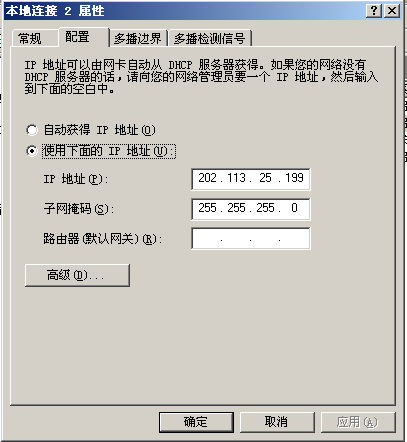
\includegraphics[width=0.6\textwidth]{3}
	\caption{TCP协议状态转换参考示意图 \label{fig:3}}
\end{figure}


\subsection{连接建立与拆除}

借鉴TCP的三次握手建立连接的思路,本次实验中的连接建立过程也是基于server和client的三次握手通信,假设用户端发送了连接建立请求,服务端会回送一条连接建立响应,表明自己受到了该用户端的连接请求,同一建立连接,之后用户端接收到连接建立响应之后,发送一条确认报文到服务端确认连接已经建立,开始数据通信过程(在本实验的数据通信过程之前还需要进行用户授权的验证过程)。相关的TCP连接示意图如\figref{fig:1} 与\figref{fig:2}所示。 

\begin{figure}[htbp]
	\centering
	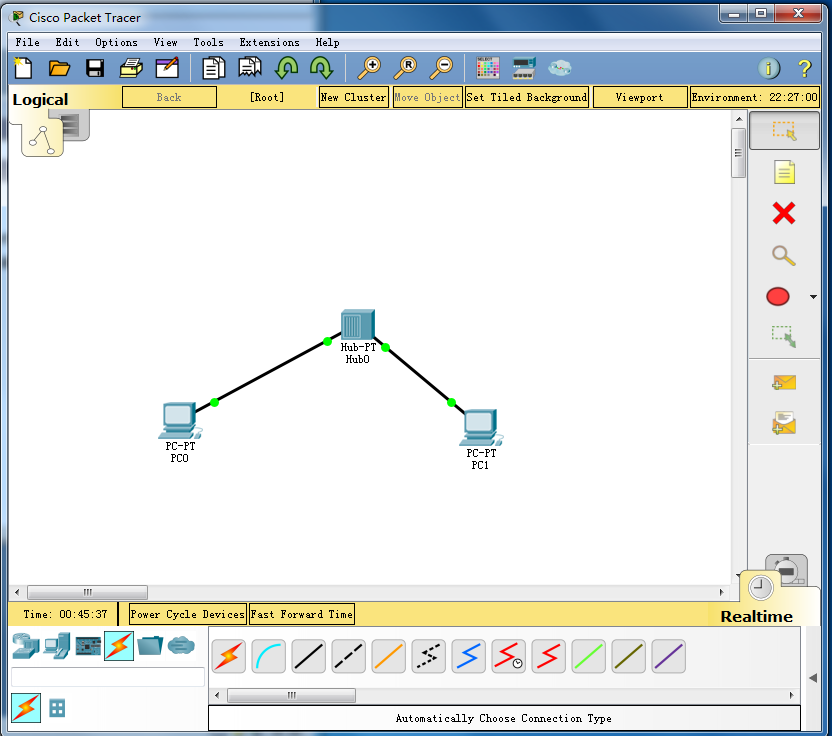
\includegraphics[width=0.6\textwidth]{1}
	\caption{TCP连接建立示意图 \label{fig:1}}
\end{figure}%

\begin{figure}[htbp]
	\centering
	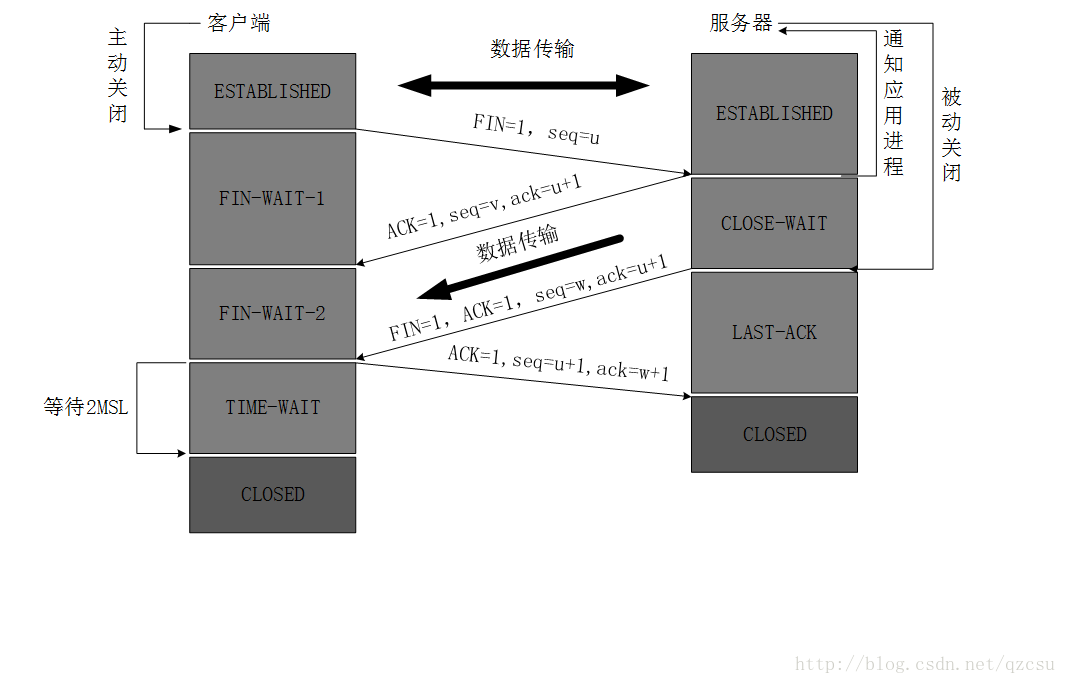
\includegraphics[width=0.6\textwidth]{2}
	\caption{TCP连接拆除示意图 \label{fig:2}}
\end{figure}%

\subsection{差错检验}
由于UCP协议中的差错校验功能属于可选项,为了进一步提高可靠性,在本次实验中,自行设计了数据报文的报文首部,在其中添加了对数据字段所有数据的校验和计算的结果存储位置,在数据报文的接收端首先会对数据进行校验和的计算检查工作,确认无误之后才会进一步进行分析,否则将抛弃出错报文。


\subsection{重传机制}

在数据传输过程中,数据报丢失的标志可以简单分为两种,即超时丢包和重复确认的出现,所以在本次实验中也实现了这两个部分,即超过了预先设定的数据响应时间即重传报文,如果连续接受到了三次重复序列的确认响应,则也重发尚在缓冲区中的所有报文,重发次数超过限制则将其清除出发送缓冲区,并进行错误报告,如果顺利接受到对应的ACK响应则缓冲报文退出缓冲区。

\subsection{连接状态维护}

由于本次实现的文件传输协议较为简单,所以不必考虑太复杂的状态,所以在本次实验的实现中,主要有系统启动、连接中、授权中、控制流交互中、文件传输中、连接断开几种状态。通过设定交互的流程将服务端和客户端的状态限定在这几个状态之中,用户的行为或命令能够触发系统的状态发生转移从而完成相应的功能。同时状态的设定也能够更好的完成整个系统的交互设计和安全性构建,使得系统更加的稳定和可靠。

\subsection{并发传输}

实验要求在数据传输中能够实现用户的并发下载,在这一部分的设计上,我主要考虑使用多线程实现,同时通过用户端和服务端协商同时传输的各文件ID编码,通过ID编码区分非按序到达的文件数据报文,然后通过归并同样的ID标识的文件数据包得到完整的传输文件,从而实现文件下载功能实现,由于采用多线程实现,各个文件的传输是非按序执行的,所以较小的文件能够很快的传输完成。

\section{实验具体实现}

基于上述的实现思路,实验中有五个主要的方面需要进行考虑,需要实现的重要功能为连接状态的建立和维护,可靠的数据传输机制以及并发的数据传输支持。以下主要从这三个主要的功能方面进行详细的叙述。

程序实现的主界面效果如\figref{fig:5}以及\figref{fig:6}所示:

\begin{figure}[H]
	\centering
	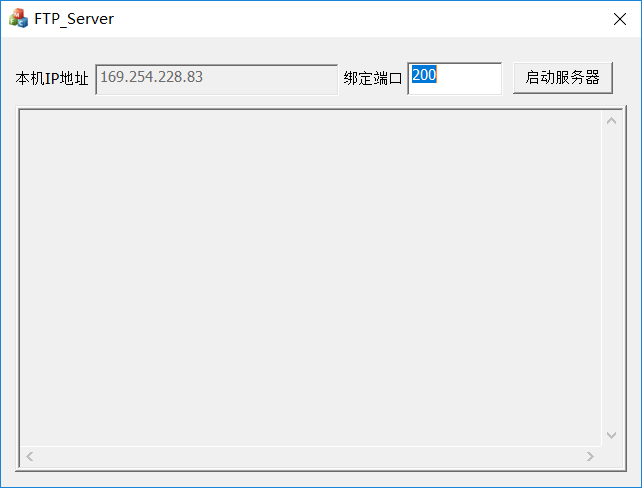
\includegraphics[width=0.6\textwidth]{5}
	\caption{Server主界面效果\label{fig:5}}
\end{figure}

\begin{figure}[H]
	\centering
	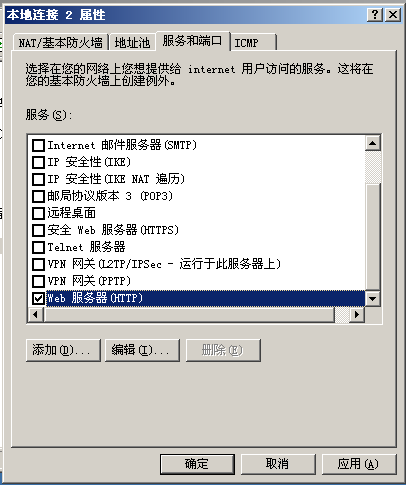
\includegraphics[width=0.6\textwidth]{6}
	\caption{CLient主界面效果 \label{fig:6}}
\end{figure}

为了实现上述思路中的主要功能,需要设计报文的自定义头部,以及在发送数据时根据参数自动生成头部,结合数据部分一同发送出去,自定义报文头部的示意图如 \figref{fig:4}所示:

\begin{figure}[H]
	\centering
	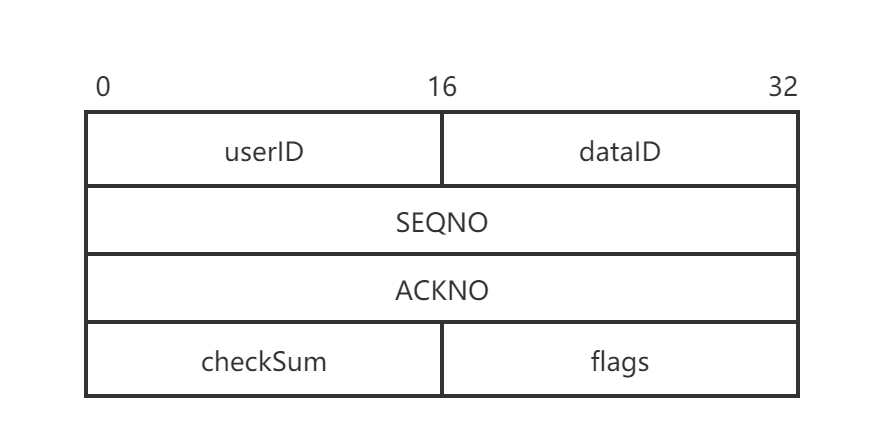
\includegraphics[width=0.6\textwidth]{4}
	\caption{自定义报文头部示意图 \label{fig:4}}
\end{figure}

相关的代码设置为如下所示:

\begin{lstlisting}[language = C++, numbers=left, 
numberstyle=\tiny,keywordstyle=\color{blue!70},
commentstyle=\color{red!50!green!50!blue!50},frame=shadowbox,
rulesepcolor=\color{red!20!green!20!blue!20},basicstyle=\ttfamily]
//定义FTP协议报文格式
typedef struct FTPHeader_t {	//FTP报文首部
WORD UserID;				//用户标识,区别不同的用户
WORD DataID;				//数据包标识,识别同一个包的不同数据报文
DWORD SEQNO;					//发送序列号
DWORD ACKNO;					//确认序列号
WORD CheckSum;				//校验和,由于文件较大,只对头部数据以及IP地址和端口数据做校验
WORD Flags;					//标志位字段
}FrameHeader_t;

\end{lstlisting}

生成报文头部并进行数据发送的函数如下所示,通过接受参数并将参数中的相关值赋值给报文头部的相应位置,然后通过SendTo将报文发送到目的主机,简化代码复杂度,提高代码复用率。


\begin{lstlisting}[language = C++, numbers=left, 
numberstyle=\tiny,keywordstyle=\color{blue!70},
commentstyle=\color{red!50!green!50!blue!50},frame=shadowbox,
rulesepcolor=\color{red!20!green!20!blue!20},basicstyle=\ttfamily]
//发送数据包函数
bool sendFTPPacket(CAsyncSocket* socket,			//发送套接字
CString toIP,									//发送至IP
UINT toPort,									//发送至端口
u_char* sendData,								//发送数据首地址
int dataLen,									//发送数据长度
WORD userID ,									//用户ID标识
WORD dataID ,									//数据字段标识
DWORD seq ,										//发送序列号
DWORD ack ,										//确认序列号
WORD flags)										//标识位
{
int totalLen = dataLen + sizeof(FTPHeader_t);
assert(totalLen <= 1472);							//保证传输的其他数据长度小于剩余的传输空间1472 - 16 = 1456字节
u_char* buffer = new u_char[totalLen];					//考虑到MTU的大小,将UDP发送数据的最大大小限制在1472字节以内
FTPHeader_t* FTPH = (FTPHeader_t*)(buffer);
FTPH->UserID = userID;
FTPH->DataID = dataID;
FTPH->Flags = flags;
FTPH->SEQNO = seq;
FTPH->ACKNO = ack;
copyData(sendData, (buffer + sizeof(FTPHeader_t)), dataLen);	//复制数据到发送缓冲中
FTPH->CheckSum = 0;												//先将校验和置位0
FTPH->CheckSum = ChecksumCompute((unsigned short*)buffer, totalLen);

int flg = socket->SendTo(buffer, totalLen, toPort, toIP, 0);	//发送数据报
if (flg < 0)
{
return false;
}
//如果数据包只有包头,没有数据,不用添加到发送缓冲区
if (totalLen - sizeof(FTPHeader_t) == 0)
{
return true;
}
//每发送一个数据包,需要把数据包存入数据缓冲区,并添加计时器
SendPacket_t* packet = new SendPacket_t;
copyData(buffer,packet->PktData, totalLen);
packet->len = totalLen;
packet->TargetIP = toIP;
packet->TargetPort = toPort;
packet->Timer = ((ConnectSocket*)(socket))->getTimerID();
packet->ResendTime = 0;												//重发次数初始化为0
((ConnectSocket*)(socket))->sendPKT_list.AddTail(packet);			//加入缓冲区	
assert(newTimer(packet->Timer));									//添加计时器
return true;
}

\end{lstlisting}


\subsection{连接状态建立和维护}

依据上述的实现思路,模仿TCP协议进行链接状态的建立和关系,在程序中设定了一些状态的宏定义如下所示:

\begin{lstlisting}[language = C++, numbers=left, 
numberstyle=\tiny,keywordstyle=\color{blue!70},
commentstyle=\color{red!50!green!50!blue!50},frame=shadowbox,
rulesepcolor=\color{red!20!green!20!blue!20},basicstyle=\ttfamily]
//描述连接状态
#define start        0		//启动初始化状态
#define isConnecting 1		//正在进行链接
#define isCommunicating 2	//正在进行命令交互
#define isTransfer	3		//正在进行数据传输
#define sendedFIN 4			//正在进行拆除连接工作,已发送拆除连接命令
#define recvedFIN 5			//接收到服务器发送来的断开连接请求
#define finished 6			//连接已经拆除


//定义标识位宏
#define SYN 0x0001				//标识连接请求位
#define ACK 0x0002				//标识ACK位有效
#define FIN 0x0004				//标识结束连接请求位
#define RST 0x0008				//标识重置连接,立即关闭连接


//计时器限制
#define TIMERLIMITNUM 20        //缓冲区最多存在20个待发送数据包
//重发次数上限
#define RESENDTIMELIMIT 5		//重发次数上限为5次,五次重发没有收到响应,进行报错

\end{lstlisting}

上述宏定义中在服务器端和客户端均有设置,因为区别不大,在此不做区分说明,链接状态宏定义用于描述系统目前所处状态,进而可以依据不同转态执行不同的操作。标示位定义宏,用于自定义数据包头部进行状态建立和状态修改,在客户端和服务器端传输状态参数。计时器和重发上限宏定义用于可靠传输中重传机制的实现。

由于状态维护相关的设置较为分散且不易于集中讲述,所以不再赘述,在这里主要以连接建立为例结合代码进行讲解,以客户端代码为例,如下所示:

\begin{lstlisting}[language = C++, numbers=left, 
numberstyle=\tiny,keywordstyle=\color{blue!70},
commentstyle=\color{red!50!green!50!blue!50},frame=shadowbox,
rulesepcolor=\color{red!20!green!20!blue!20},basicstyle=\ttfamily]
case SYN | ACK:
{
//接受到连接请求响应
if (status == isConnecting)			//接收到服务器链接请求响应
{
//保存返回的用户ID
this->userID = FTPH->UserID;
//修改连接状态为正在通信状态
this->status = isCommunicating;
//创建一个发送数据包结构体
u_char res[256] = "OK Client is ready!";
int res_len = strlen((char*)(res));
//更新发送序列号
Seq += res_len;
//回送一个ACK报文,确认已收到连接返回响应,确认建立连接
sendFTPPacket(this, serverIP, serverPort, res, res_len, userID, 0, Seq, Ack, ACK);
//日志记录 
Dlg->log(((CString)Data).Left(byteLen - sizeof(FTPHeader_t)));
}
break;
}
\end{lstlisting}

如上述代码所示,客户端建立套接字监听端口之后,如果点击发送建立连接的按钮,则会触发向服务器端发送连接建立请求的报文,服务器端接收到连接建立请求之后,会回送确认报文,确认报文中的头部标示位为SYN|ACK,通过判断该标识位区分报文的意图,进而执行相应的操作,在这里客户端执行的操作是回送一个ACK确认报文,表明连接建立成功。

\subsection{可靠数据传输机制}

可靠的数据传输机制在本实验中主要有两个实现方式,一个是校验和的计算和比对,实现差错检验功能,差错检验功能主要依靠报文头部中的校验和为和校验和计算函数,校验和计算函数如下所示:

\begin{lstlisting}[language = C++, numbers=left, 
numberstyle=\tiny,keywordstyle=\color{blue!70},
commentstyle=\color{red!50!green!50!blue!50},frame=shadowbox,
rulesepcolor=\color{red!20!green!20!blue!20},basicstyle=\ttfamily]
// 计算校验和
unsigned short ChecksumCompute(unsigned short * buffer, int size)
{
// 32位,延迟进位
unsigned long cksum = 0;
while (size > 1)
{
cksum += *buffer++;
// 16位相加
size -= sizeof(unsigned short);
}
if (size)
{
// 最后可能有单独8位
cksum += *(unsigned char *)buffer;
}
// 将高16位进位加至低16位
cksum = (cksum >> 16) + (cksum & 0xffff);
cksum += (cksum >> 16);
// 取反
return (unsigned short)(~cksum);
}
\end{lstlisting}

利用校验和计算函数和校验和位,在接受到报文数据之后,提取校验和为和重新计算的校验和进行比对,如果无误则继续处理,否则丢弃报文并报告记录日志。相关代码如下所示:

\begin{lstlisting}[language = C++, numbers=left, 
numberstyle=\tiny,keywordstyle=\color{blue!70},
commentstyle=\color{red!50!green!50!blue!50},frame=shadowbox,
rulesepcolor=\color{red!20!green!20!blue!20},basicstyle=\ttfamily]
if (ChecksumCompute((unsigned short *)buffer, byteLen) != 0)			//差错检验
{
Dlg->log("数据包校验和计算错误!");
return;
}
\end{lstlisting}

另外一个实现可靠数据传输的方式为超时重传和快速重传机制,如果发送缓冲区中的数据包发送超时或者连续接收了三次冗余ACK之后重传报文,这里需要数据结构的支持,自行设计的一个发送缓冲去数据报文的数据结构定义如下:

\begin{lstlisting}[language = C++, numbers=left, 
numberstyle=\tiny,keywordstyle=\color{blue!70},
commentstyle=\color{red!50!green!50!blue!50},frame=shadowbox,
rulesepcolor=\color{red!20!green!20!blue!20},basicstyle=\ttfamily]
//发送数据包在缓冲区中的格式
typedef struct SendPacket_t {
int len;				//数据包长度
BYTE PktData[2000];		//数据包
CString TargetIP;		//目的IP地址,使用字符串格式
UINT   TargetPort;		//目的端口号
UINT_PTR Timer;			//计时器句柄
int ResendTime;			//重发次数
};
\end{lstlisting}

通过给每一个缓冲区中的报文定义一个计时器,计时器触发之后会自动重传该报文,实现超时重传功能,相关代码如下所示:

\begin{lstlisting}[language = C++, numbers=left, 
numberstyle=\tiny,keywordstyle=\color{blue!70},
commentstyle=\color{red!50!green!50!blue!50},frame=shadowbox,
rulesepcolor=\color{red!20!green!20!blue!20},basicstyle=\ttfamily]

//计时器响应函数,发送缓冲区数据超时未获答复,重传报文
void CFTP_ClientDlg::OnTimer(UINT_PTR nIDEvent)
{
// TODO: 在此添加消息处理程序代码和/或调用默认值
if (CNSocket->sendPKT_list.GetCount() == 0)
{
MessageBox("计时器错误");
return;
}
POSITION pos = CNSocket->sendPKT_list.GetHeadPosition();
while (pos != NULL)
{
if (CNSocket->sendPKT_list.GetAt(pos)->Timer == nIDEvent)
{
if (CNSocket->sendPKT_list.GetAt(pos)->ResendTime >= RESENDTIMELIMIT)		//重传次数超过上限,报错,删除重传报文
{
CString logText;
logText.Format("重传次数超限,删除报文:SEQ:", ((FTPHeader_t*)(CNSocket->sendPKT_list.GetAt(pos)->PktData))->SEQNO);
log(logText);
CNSocket->backTimerID(nIDEvent);
CNSocket->sendPKT_list.RemoveAt(pos);
break;
}
CNSocket->SendTo(CNSocket->sendPKT_list.GetAt(pos)->PktData,
CNSocket->sendPKT_list.GetAt(pos)->len,
CNSocket->sendPKT_list.GetAt(pos)->TargetPort,
CNSocket->sendPKT_list.GetAt(pos)->TargetIP);
CNSocket->sendPKT_list.GetAt(pos)->ResendTime++;		//计数器增加1
CString logText;
logText.Format("超时重传:SEQ:%d", ((FTPHeader_t*)(CNSocket->sendPKT_list.GetAt(pos)->PktData))->SEQNO);
log(logText);
break;
}
CNSocket->sendPKT_list.GetNext(pos);
}
CDialogEx::OnTimer(nIDEvent);
}
\end{lstlisting}

如果接收到了数据包的ACK确认,那么就将相应的缓冲区中的数据包从缓冲区中移除并且回收计时器的ID。如果连续接收了三次冗余ACK也会触发缓冲区中的所有报文进行重新发送的操作。

\subsection{并发文件数据传输}

并发数据传输机制依赖于报文头部定义的DATAID位,通过改为标识报文属于哪一个文件,在接收端会通过该ID进行报文的归并,组合形成相应的文件,这里也定义了数据结构进行支持,数据结构如下所示:

\begin{lstlisting}[language = C++, numbers=left, 
numberstyle=\tiny,keywordstyle=\color{blue!70},
commentstyle=\color{red!50!green!50!blue!50},frame=shadowbox,
rulesepcolor=\color{red!20!green!20!blue!20},basicstyle=\ttfamily]
typedef struct DownloadFile_t {
WORD DataID;			//文件ID
CString filename;		//文件名
u_char filecontent[10000000];	//文件内容
long long int len;		//文件内容长度
} DownloadFile_t;
\end{lstlisting}

通过该数据结构记录接受的文件数据报文,并在文件传输接收表示\text(CRCFCRCFCRCFCRCF)出现之后进行报文的归并工作,将数据写入文件,实现文件下载功能。

并发的数据传输在server端依靠一个文件传输线程控制函数实现,该函数的具体代码如下所示:


\begin{lstlisting}[language = C++, numbers=left, 
numberstyle=\tiny,keywordstyle=\color{blue!70},
commentstyle=\color{red!50!green!50!blue!50},frame=shadowbox,
rulesepcolor=\color{red!20!green!20!blue!20},basicstyle=\ttfamily]
//线程控制函数
UINT dataThread(LPVOID lpParam)
{
DownloadFile_t *pInfo = (DownloadFile_t*)lpParam;     //指向结构体的实例。
CFTP_ServerDlg*  Dlg = (CFTP_ServerDlg*)(AfxGetApp()->GetMainWnd());
//记录日志
CString t;
t.Format("启动发送文件线程%d,%s", pInfo->DataID, pInfo->filename);
// 等待互斥对象通知
WaitForSingleObject(hMutex, INFINITE);
Dlg->log(t);
// 释放互斥对象
ReleaseMutex(hMutex);
//启动数据读取
u_char* data;
long long int data_len;
readFile(pInfo->filename,data, data_len);
t.Format("%s 开始传输!文件大小:%d", pInfo->filename, data_len);
Dlg->log(t);
//Dlg->MessageBox((CString)data);
//开始发送
long long  sendedSeq = 0 ;
while (sendedSeq < data_len)
{
if (data_len - sendedSeq>=DATAMAXLEN)		//数据长度大于报文承载长度
{
// 等待互斥对象通知
WaitForSingleObject(hMutex, INFINITE);
u_char* tt = new u_char[DATAMAXLEN];
copyData(data + sendedSeq, tt, DATAMAXLEN);
pInfo->server->Seq += DATAMAXLEN;
sendFTPPacket(pInfo->server, pInfo->toIP, pInfo->port, tt, DATAMAXLEN,pInfo->server->userID, pInfo->DataID, pInfo->server->Seq, pInfo->server->Ack, ACK);
sendedSeq += DATAMAXLEN;
t.Format("%s 传输进度:%d/%d", pInfo->filename,sendedSeq, data_len);
Dlg->log(t);
// 释放互斥对象
ReleaseMutex(hMutex);
}
else {
// 等待互斥对象通知
WaitForSingleObject(hMutex, INFINITE);
u_char* tt = new u_char[data_len - sendedSeq];
copyData(data + sendedSeq, tt, data_len - sendedSeq);
pInfo->server->Seq += data_len - sendedSeq;
sendFTPPacket(pInfo->server, pInfo->toIP, pInfo->port, tt, data_len - sendedSeq, pInfo->server->userID, pInfo->DataID, pInfo->server->Seq, pInfo->server->Ack, ACK);
sendedSeq += data_len - sendedSeq;
t.Format("%s 传输进度:%d/%d", pInfo->filename, sendedSeq, data_len);
Dlg->log(t);
// 释放互斥对象
ReleaseMutex(hMutex);
}
}
// 等待互斥对象通知
WaitForSingleObject(hMutex, INFINITE);
u_char end[123] = "\r\n\r\n\r\n\r\n";
int str_len = strlen((char *)end);
pInfo->server->Seq += str_len;
sendFTPPacket(pInfo->server, pInfo->toIP, pInfo->port, end,str_len, pInfo->server->userID, pInfo->DataID, pInfo->server->Seq, pInfo->server->Ack, ACK);
// 释放互斥对象
ReleaseMutex(hMutex);
t.Format("%s 文件传输完毕!文件大小:%d", pInfo->filename, data_len);
// 等待互斥对象通知
WaitForSingleObject(hMutex, INFINITE);
Dlg->log(t);
// 释放互斥对象
ReleaseMutex(hMutex);
return 0;
}
\end{lstlisting}

当server端接收到来自于用户的多个文件下载请求,它会首先解析报文中的下载文件,并按照预先预定好的的顺序(发送顺序)作为文件的DATAID,之后的该文件分开的所有报文头部均需要添加该dataID的值,以实现区分的作用。在接收端按照dataID 归类之后,就能够实现多文件并发下载的功能了。


\section{实验效果演示}
 
本次实验编写的程序能够实现文件传输协议的许多基本功能,以下为本次实验的的主要功能演示截图。

\subsection{建立连接效果演示}

\begin{figure}[H]
	\centering
	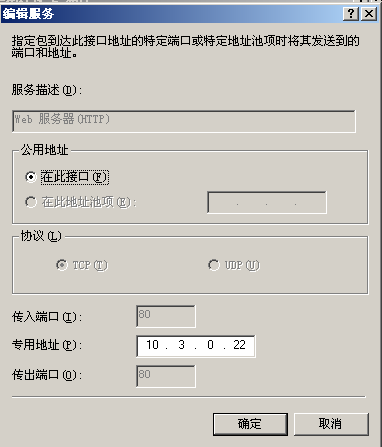
\includegraphics[width=0.40\textwidth]{7}
	\caption{连接建立演示\label{fig:7}}
\end{figure}


\subsection{用户授权验证演示}
由于预设了一个用户test(密码为test),可以尝试直接登录。
\begin{figure}[H]
	\centering
	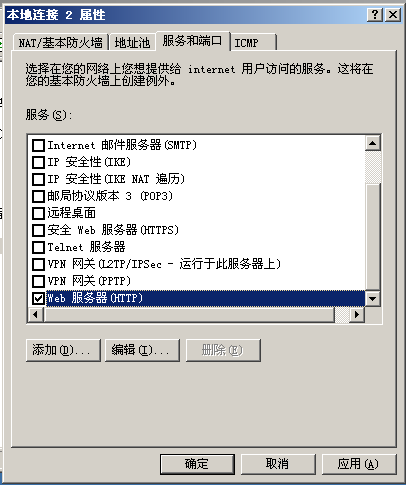
\includegraphics[width=0.40\textwidth]{6}
	\caption{用户授权登录演示 \label{fig:6}}
\end{figure}
如果输入错误密码会进行提示,如果输入不存在的用户名,系统视为注册新用户,会创建一个空的用户空间并且返回。

\subsection{获取远程目录演示}
通过LIST命令获取远程目录并显示。
\begin{figure}[H]
	\centering
	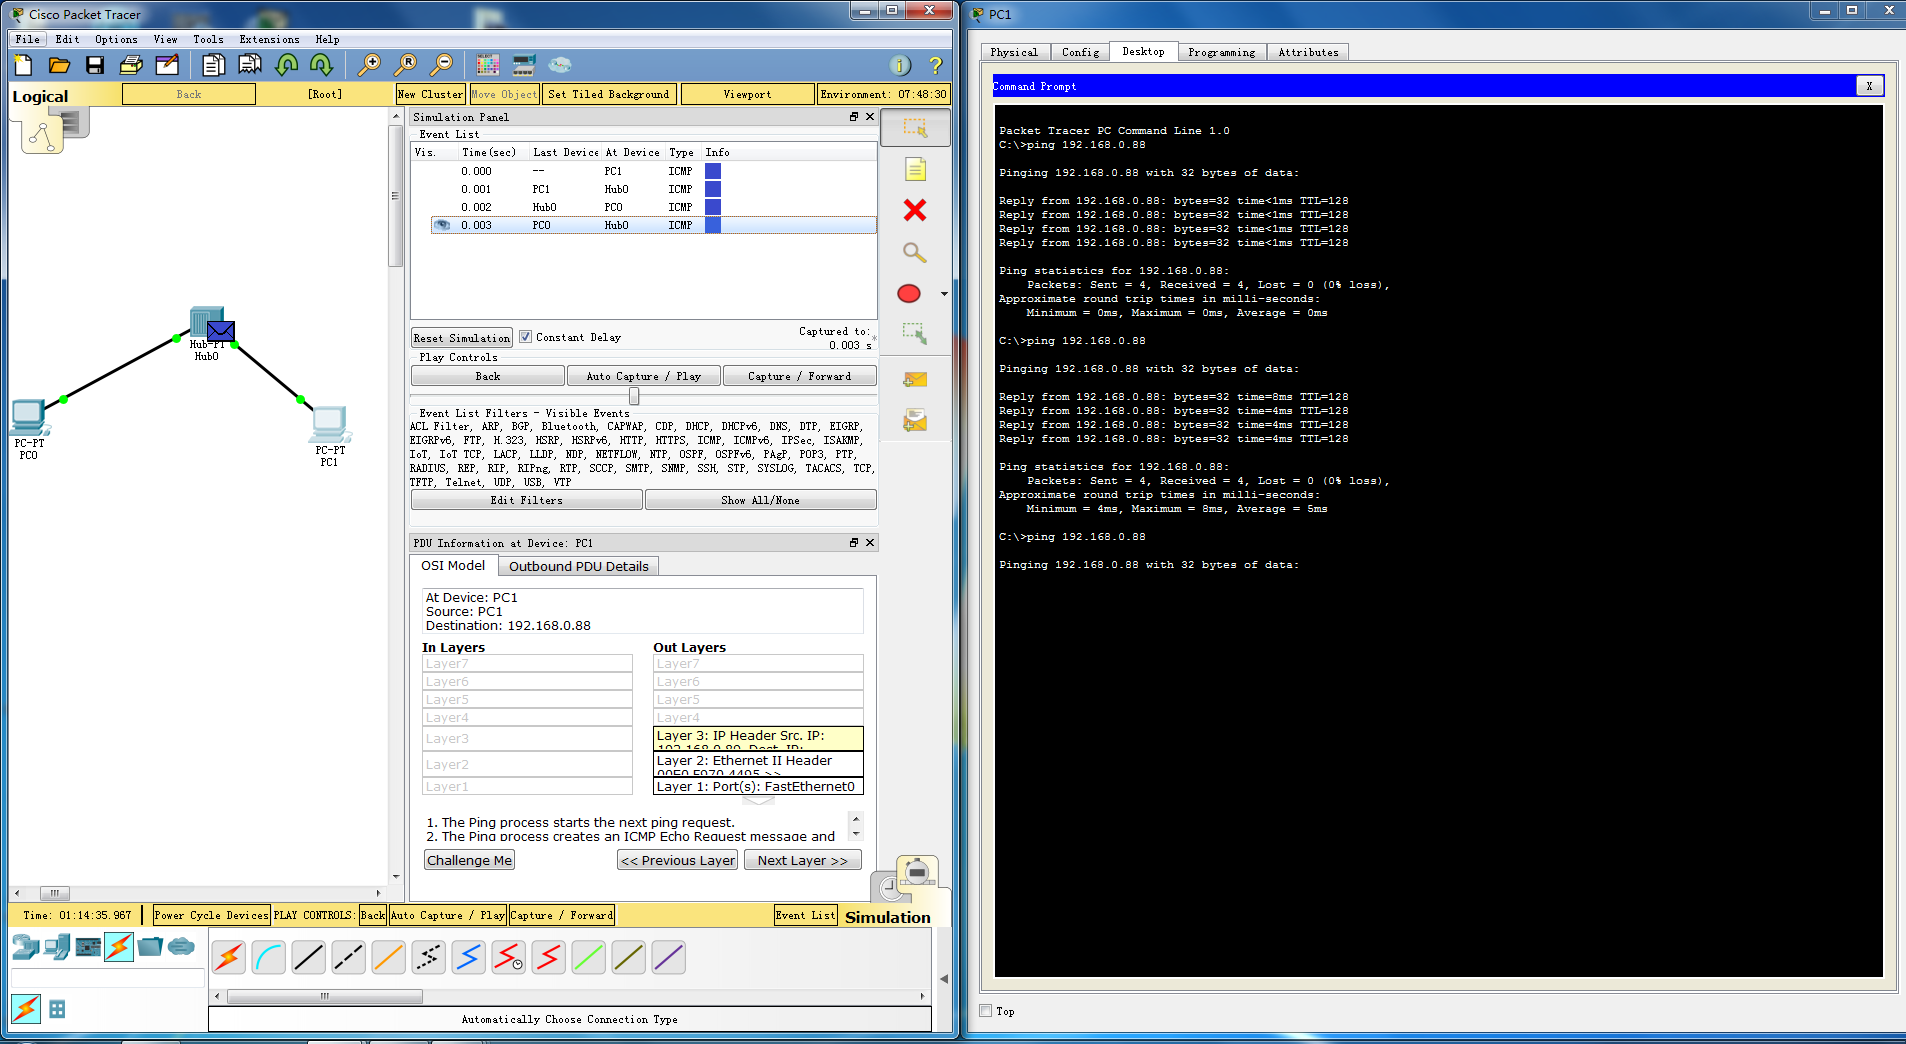
\includegraphics[width=0.35\textwidth]{9}
	\caption{获取远程目录演示 \label{fig:9}}
\end{figure}

\subsection{并发下载文件演示}
通过RETR命令下载文件,可以通过双击文件树显示窗口,添加需要下载的文件,注意不要直接输入下载文件的名字。

\begin{figure}[H]
	\centering
	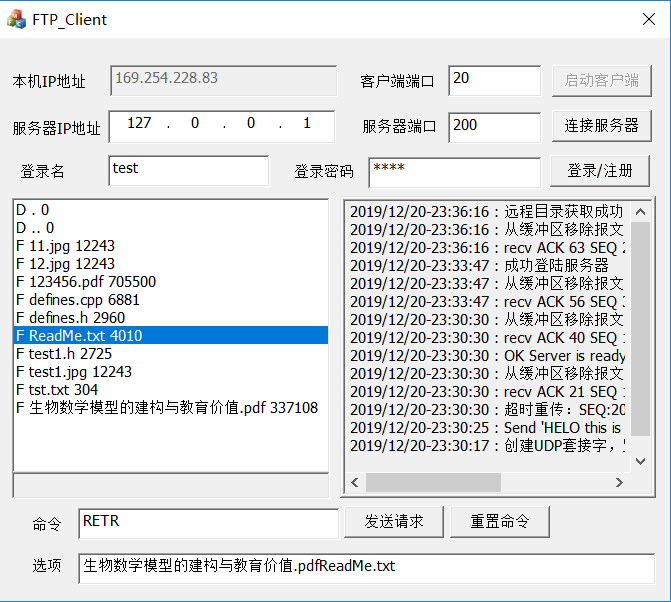
\includegraphics[width=0.5\textwidth]{10}
	\caption{并发下载命令演示 \label{fig:10}}
\end{figure}

\begin{figure}[H]
	\centering
	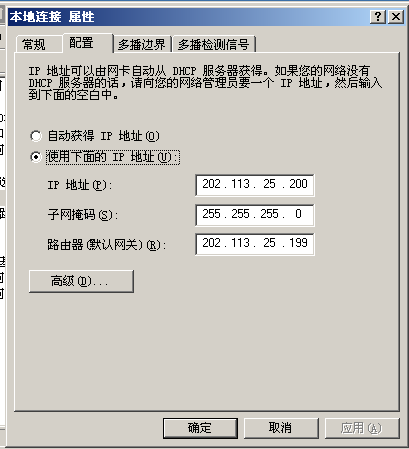
\includegraphics[width=0.5\textwidth]{11}
	
	\caption{并发下载结果显示1 \label{fig:11}}
\end{figure}

\begin{figure}[H]
	\centering
	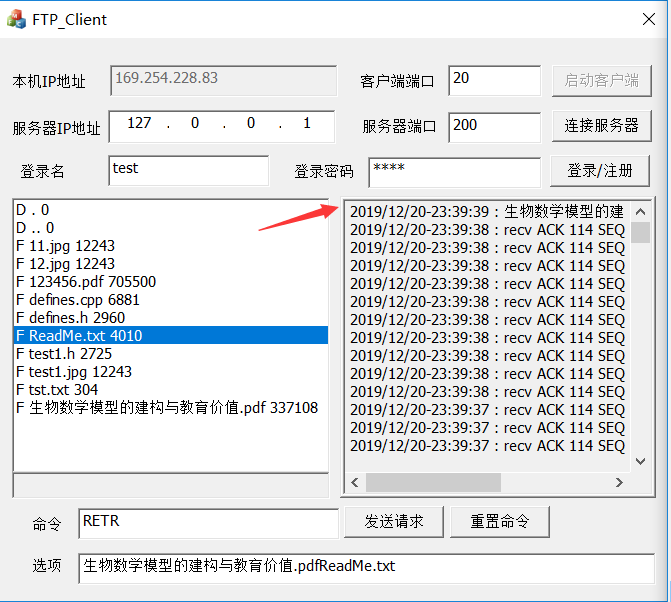
\includegraphics[width=0.5\textwidth]{12}
	
	\caption{并发下载结果显示2 \label{fig:12}}
\end{figure}

由于先添加大的文件,如果非并发则大文件因先下载完成,但是从演示结果看到确实是并发下载的结果。

\subsection{创建远程目录演示}
通过MDIR命令创建远程目录,然后通过LIST命令获取远程目录可以看到执行成功。

\begin{figure}[H]
	\centering
	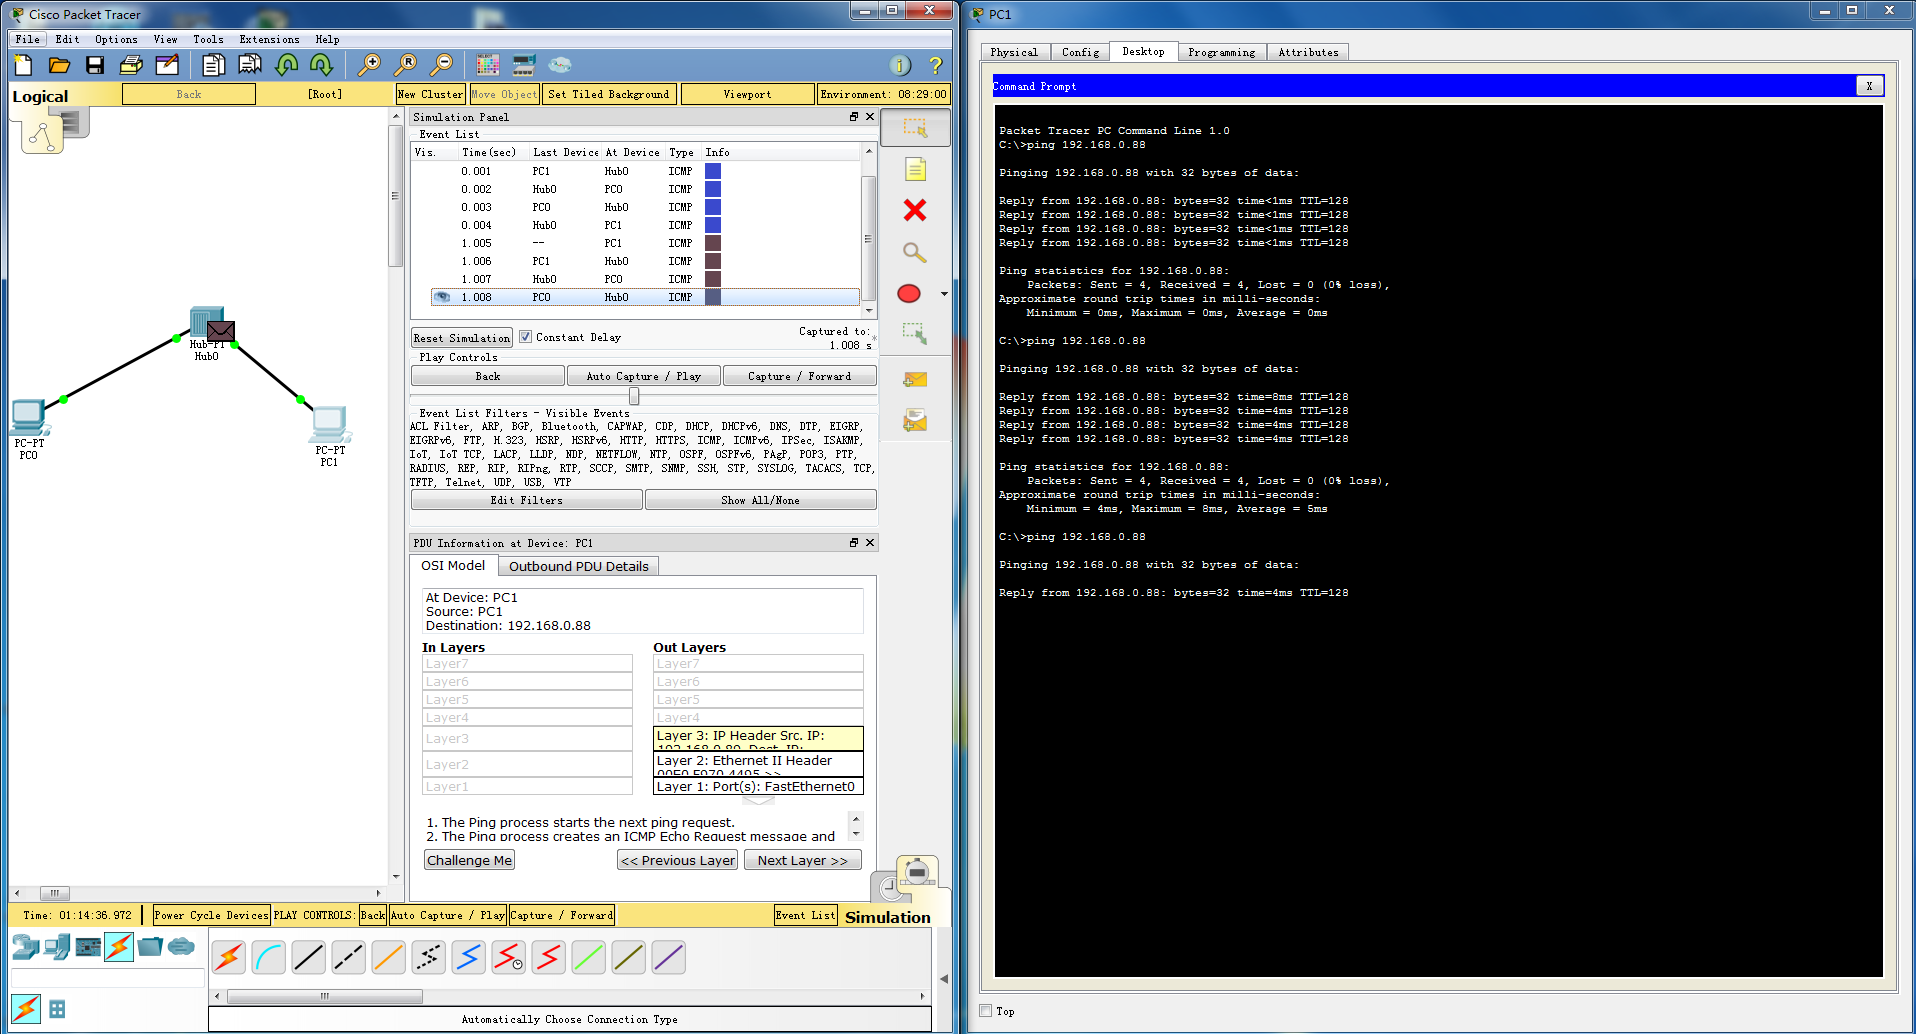
\includegraphics[width=0.5\textwidth]{13}
	
	\caption{创建远程目录演示 \label{fig:13}}
\end{figure}

\subsection{删除远程目录/文件演示}
通过DELE命令可以删除远程文件或者目录。

\begin{figure}[H]
	\centering
	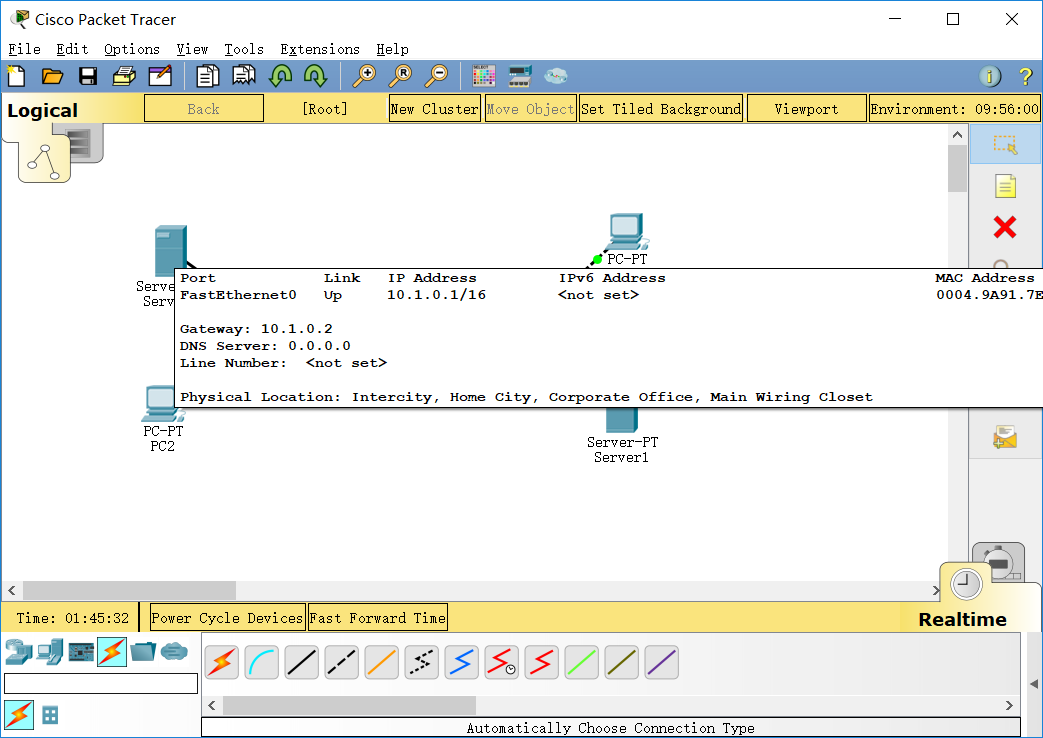
\includegraphics[width=0.6\textwidth]{14}
	
	\caption{删除远程目录/文件演示 \label{fig:14}}
\end{figure}

\subsection{断开连接演示}
通过EXIT命令断开连接。

\begin{figure}[H]
	\centering
	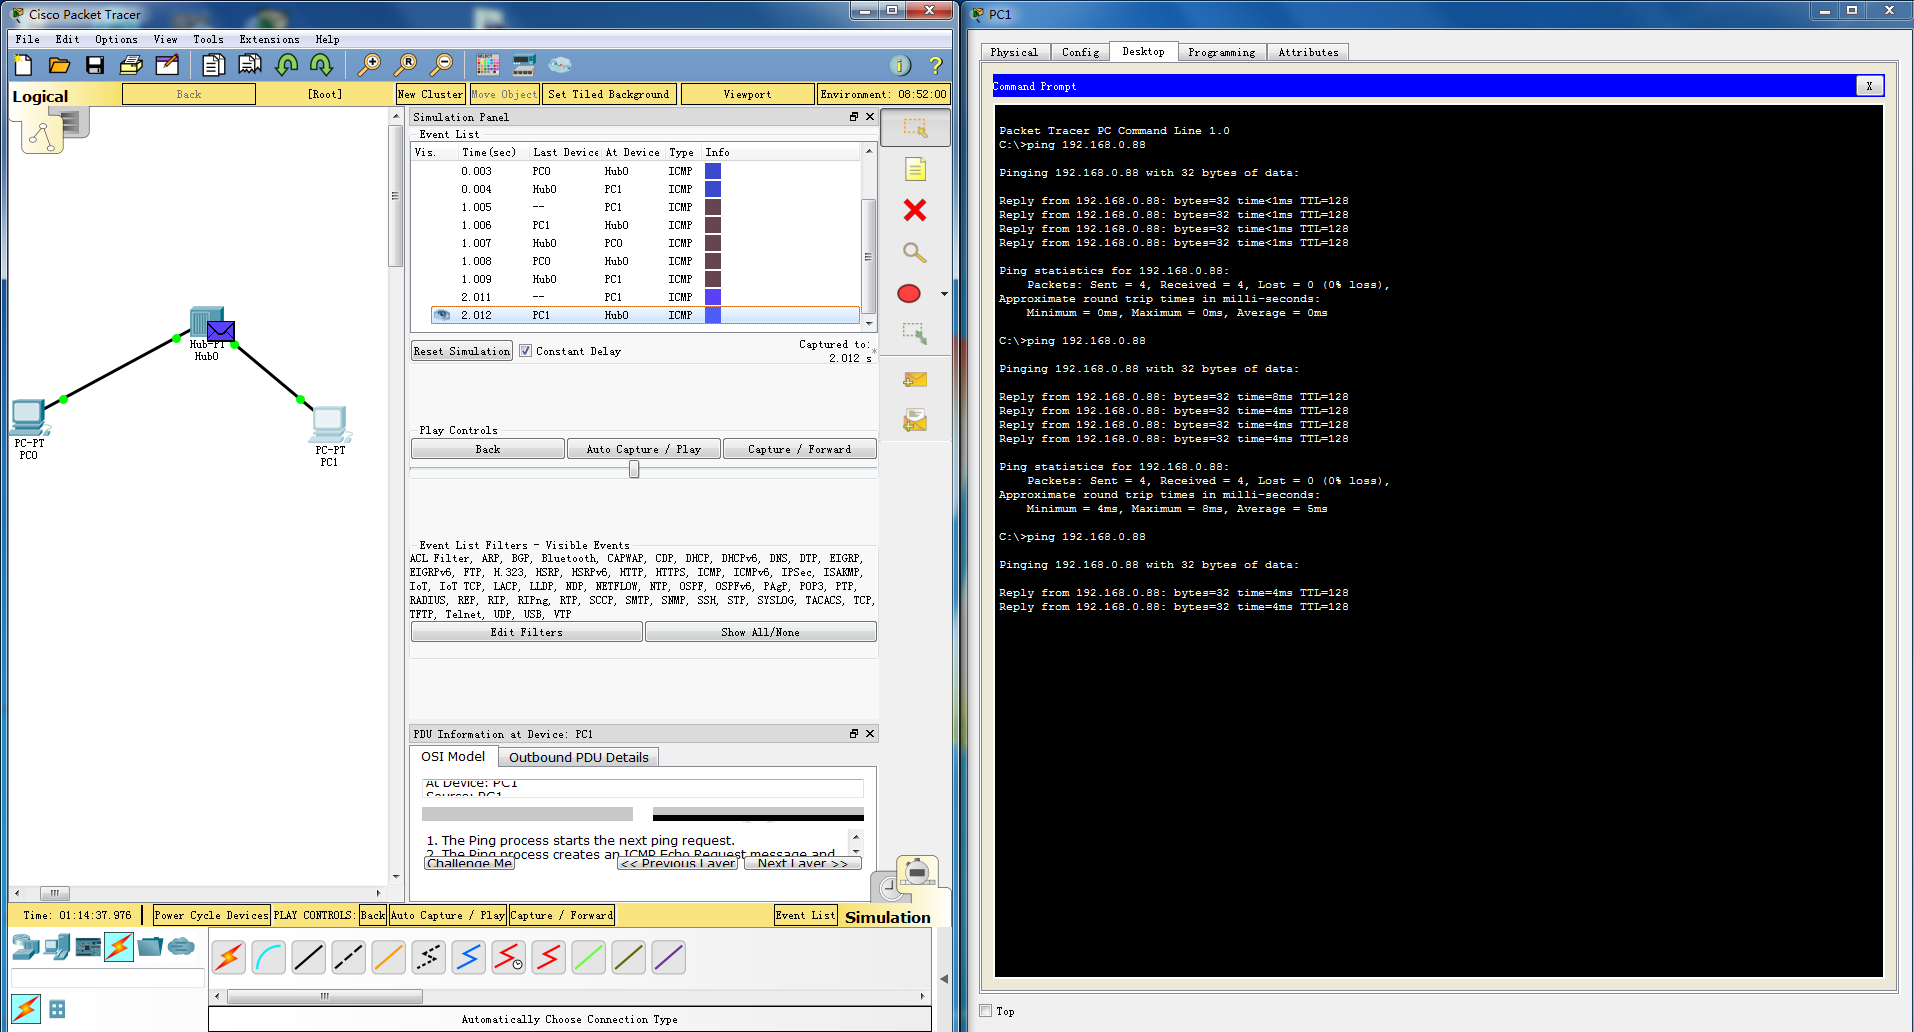
\includegraphics[width=0.6\textwidth]{15}
	
	\caption{断开连接演示 \label{fig:15}}
\end{figure}



\section{总结与思考}
通过这次实现应用层的类FTP文件传输协议,我对于协议的本质有了更加深刻的认识,理解了UDP协议和应用层协议的重要作用,以及实现的流程和重点内容,尤其是多线程编程的练习进一步锻炼了我的编程能力,在实现系统的过程中不断的改正错误,使得系统逐渐变得更加的流畅和完善,虽然最终有部分的缺憾但是总体上还是让我十分满意的。

这次的实验无论是对我的动手实践能力还是理论知识的认识都有很大的提升作用,不过花了很多的时间,临近期末确实有些忙了,所有在程序中还是有部分问题存在,但是已经没有足够的时间让我去完善它了。经过这次的实验,感觉自己的编程能力还需要进一步的提升,对知识的运用还要更加的灵活。


% 如果想修改参考文献样式(非国标),请把下行取消注释,并换成合适的样式(比如 unsrt,plain 样式)。
%\bibliographystyle{aer}
%\bibliography{wpref}

\end{document}
